\cleardoublepage

\chapter{Nodo}
\label{makereference2}

\section{Introducción}
\label{makereference2.1}
Como hemos comentado anteriormente el \textbf{nodo} es quien recoge los datos meteorológicos escogidos y los envía al \textbf{servidor} de datos.

Se ha implementado con una \textbf{Raspberry Pi modelo 3} como placa programable y los sensores DHT22 para la medición de la temperatura y humedad y un piranómetro SP-212 para medir la irradiación solar. Ver imagen \ref{node-diagram}

La parte software del nodo ha sido implementada en \textbf{Python}.

\section{Qué variables medir}
\label{makereference2.2}
%--- http://www.pveducation.org/pvcdrom/2-properties-sunlight/solar-radiation-earths-surface

La \textbf{radiación solar} varía debido a diversos factores, como los efectos atmosféricos, las variaciones locales en la atmósfera como el vapor de agua, las nubes y la contaminación, otros como la latitud y la estación del año y la hora del día.

%--- https://www.imn.ac.cr/documents/10179/27818/factores-influyen-radiac-UV.pdf/187e5ea7-7c11-4ed7-955b-4e35c2f0ebf1

Por ejemplo, la \textbf{latitud} influye en la cantidad de radiación solar que llega a la superficie; por otro lado, la radiación disminuirá cuanta más cantidad de nubes y más alta sea la \textbf{humedad}. Al contrario pasará con la \textbf{temperatura}, cuanto más altas sean las temperaturas mayor será la radiación. Otro factor que influye a la hora de medir la radiación, es el tipo de \textbf{superficie}, porque la reflexión de los rayos varía según el tipo. En la nieve se refleja un 85 por ciento, al contrario del asfalto que solo un 2 por ciento.

En este proyecto, se recogen solo muestras de radiación solar, temperatura y humedad por ser las más relevantes para nuestro modelo.

\section{Elementos hardware utilizados}
\label{makereference2.3}

\subsection{Raspberry Pi 3 modelo}
\label{makereference2.3.1}

Raspberry Pi es un microcontrolador, un computador de placa reducida \ref{rasp}. Con él se pueden controlar distintos componentes electrónicos a través de los pines que expone y combinarlo con la potencia y versatilidad de un sistema operativo.

\begin{figure}[htb]
	\begin{center}
		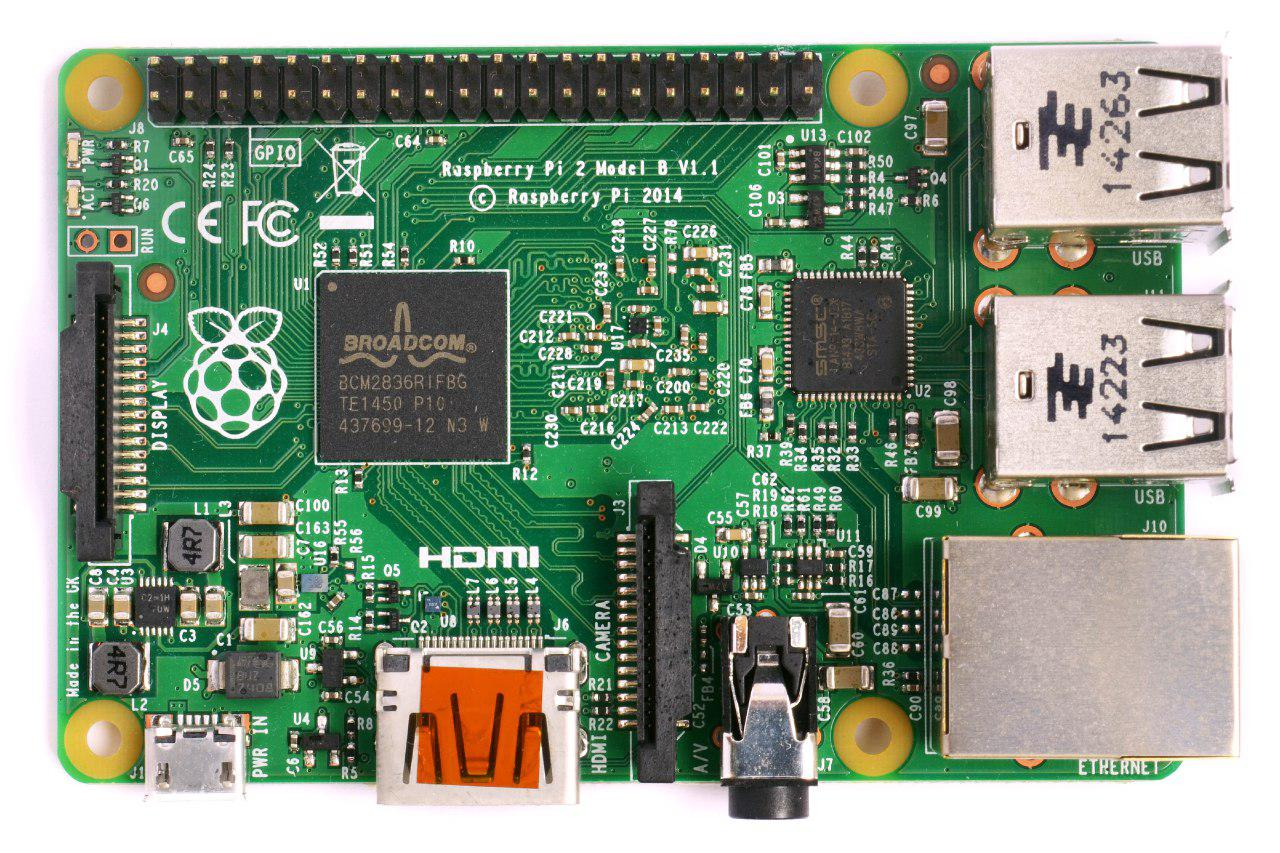
\includegraphics[height=5cm]{figures/Raspberry_Pi.jpg}
		\caption{Raspberry Pi Modelo 2b [Fuente: \href{https://www.raspberrypi.org}{Raspberry Pi}]}
	\end{center}
	
	\label{rasp}
\end{figure}

Raspberry proporciona el sistema operativo oficial llamado Raspbian, una distribución de Debian. También soporta otros sistemas operativos.
 
Fue creado en 2006, en la Universidad de Cambridge, con el fin de fomentar la enseñanza en las escuela de ciencias de la computación, pero hasta 2012 no salió al mercado.

Existen distintos modelos de Raspberry Pi, desde la Raspberry Pi 1 Modelo A hasta la Raspberry Pi 3 Modelo B \ref{types}.
En nuestro proyecto hemos usado una Raspberry Pi 3 modelo B, con su sistema operativo oficial, Raspbian.

Se ha decidido utilizar este microcontrolador en el proyecto debido a su facilidad de manejo gracias a que cuenta con un sistema operativo y por ser relativamente barato para realizar un prototipo. Además cuenta con un gran comunidad detrás que trabaja en el desarrollo de nuevas guías y librerías para facilitar el desarrollo. (\cite{ARP:RaspberryPi:2017})

\begin{figure}[htb]
	\begin{center}
		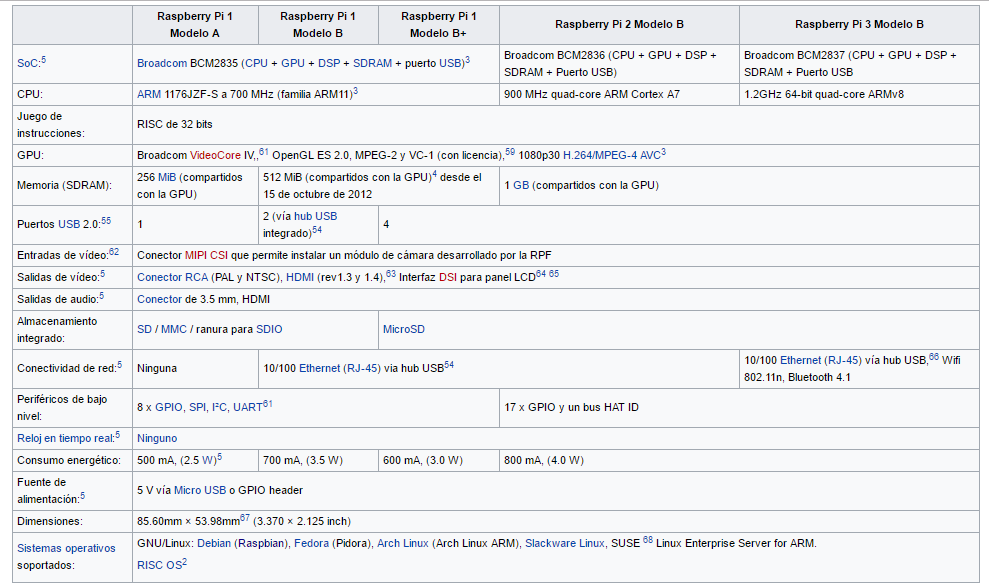
\includegraphics[width=17cm,height=12cm]{figures/Cuadro_Tipos_Raspberry.png}
		\caption{Cuadro comparativo de las especificaciones técnicas [Fuente: \href{www.wikipedia.org}{Wikipedia}]}
	\end{center}

	\label{types}
\end{figure}

\subsection{Sensor de temperatura y humedad}
\label{makereference2.3.2}

A la Raspberry se le conectan dos sensores, uno de temperatura y humedad y un piranómetro del cual hablaremos más tarde. Ambos para recoger los datos meteorológicos que necesitamos para nuestro modelo.

Para medir la temperatura y la humedad hemos utilizado un solo componente que recoge ambas muestras. El modelo escogido ha sido el sensor \textbf{DHT22}. (\cite{ARP:Adafruit:2017})

Algunas de las características de este sensor y en especial de este modelo (ya que tambien existe el modelo DHT11 de la misma marca) son que tiene una precisión de 0.5ºC para medir la temperatura, y entre un 2 y un 5 por ciento para la humedad. Ademas recogen dos muestras por segundo. Este sensor no es un sensor de alta precisión, pero es suficiente para nuestro proyecto, además de tener un precio muy económico. Ver imágen \ref{sensor}.

La comunicación entre el sensor y la Raspberry se realiza a través de un pin \textbf{GPIO} (General Purpose Input/Output, Entrada/Salida de Propósito General) que es un pin de propósito general. Estos pines pueden ser de entrada o de salida, y reciben y envían valores binarios de un bit.

En el \href{https://cdn-shop.adafruit.com/datasheets/Digital+humidity+and+temperature+sensor+AM2302.pdf}{datasheet} del sensor viene definido el proceso de comunicación entre este y la Raspberry. Para ello, el microcontrolador (Raspberry en nuestro caso) envía una señal de arranque para que el sensor cambie del estado ``standby'' al estado ``running''. Al terminar de enviar dicha señal, el sensor envía una respuesta de 40 bits que contiene la información relativa a la humedad (16 bits), a la temperatura (16 bits) y un checksum (8 bits) para comprobar que se ha enviado correctamente. Ver imagen \ref{DHT22comunication}.

El envío de estos bits sucede de la siguiente forma: el sensor envía una señal ``baja'' ("0") que indica el inicio de la transmisión de un bit. Seguidamente envía una señal ``alta'' (``1''). Si la transmisión de esta corriente dura más de $ 50 \mu $ s indica que se ha transmitido un 1, en caso contrario, se quiso transmitir un 0.

\begin{figure}[htb]
	
	\begin{center}
		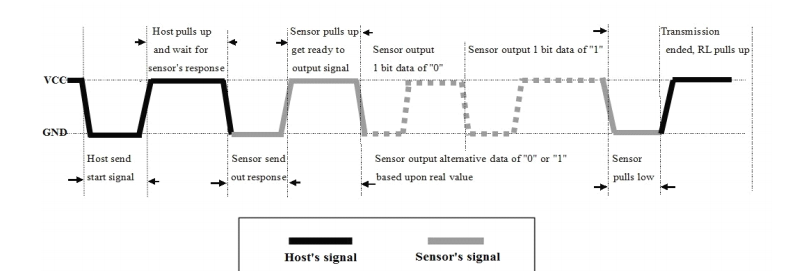
\includegraphics[width=15cm]{figures/DTH22comunicationdiagram.png}
		\caption{Diagrama de comunicación del sensor DHT22 [Fuente: \href{https://cdn-shop.adafruit.com/datasheets/Digital+humidity+and+temperature+sensor+AM2302.pdf}{Adafruit}]}
	\end{center}
	
	\label{DHT22comunication}
\end{figure} 

 \begin{figure}[htb]
	
	\begin{center}
		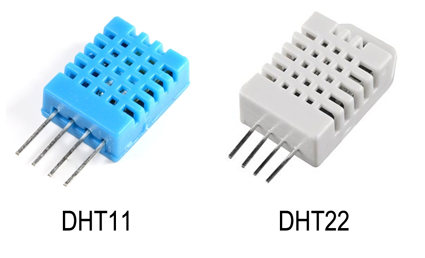
\includegraphics[width=10cm,height=7cm]{figures/sensorTemperaturaHumedad.png}
		\caption{Sensores de temperatura y humedad DHT11 y DHT22 [Fuente: \href{https://cdn-shop.adafruit.com/datasheets/Digital+humidity+and+temperature+sensor+AM2302.pdf}{Adafruit}]}
	\end{center}
	
	\label{sensor}
\end{figure} 

\subsection{Piranómetro y ADC}
\label{makereference2.3.3}
Para recoger la cantidad de irradiación solar se utiliza un piranómetro. En este proyecto se ha utilizado el modelo \href{https://www.apogeeinstruments.co.uk/content/SP-212-215-manual.pdf}{SP-212}. Este sensor es analógico es decir, la señal que envía es un voltaje variable con el cual indica la cantidad de irradiación que recoge. (\cite{ARP:Apogee:2017}).

Para poder leer esa información con un microcontrolador es necesario hacer una conversión a digital. Para ello se utiliza un conversor analógico-digital o por sus siglas en inglés \textbf{ADC}.

El \textbf{ADC} utilizado en este proyecto ha sido el \href{https://cdn-shop.adafruit.com/datasheets/MCP3008.pdf}{MCP3008}. Es un conversor de 10 bits por lo que permite codificar entre 0 y 1024, suficiente para este proyecto. Se comunica con la Raspberry a través del puerto \textbf{SPI}. (\cite{ARP:Adafruit:2017})

\textbf{SPI} es un estándar de comunicación en serie, maestro/esclavo, regulado por un reloj. Incluye 4 señales: reloj (SCLK), salida de datos del maestro y entrada de datos al esclavo (MOSI), salida de datos del esclavo y entrada al maestro (MISO) y otra para Para seleccionar un esclavo, o para que el maestro le diga al esclavo que se active (SS/Select).

Con cada pulso de reloj el maestro envía un bit. Para que empiece la transmisión el Master baja la señal SS/Select a cero, con esto el Slave se activa y empieza la transmisión, con un pulso de reloj al mismo tiempo que el primer bit es leído.

Raspberry cuenta con unos pines para la comunicación a través de SPI lo que facilita el uso de este tipo de componentes.

\section{Componentes software y librerías externas}
\label{makereference2.4}
El software a través del cual controlar el nodo ha sido escrito en Python2.7. Su punto de entrada es el archivo ``solar\_node.py''.

Se puede ejecutar a través de la consola de comandos con el comando ``python solar\_node.py''

Este programa tiene dos partes importantes: recoger los datos y enviarlos al servidor de datos. Para ello utilizamos varias librerías ya existentes.

Los datos recogidos serán almacenados en registros para evitar la pérdida de datos. Estos registros (o ``logs'') son almacenados en archivos diarios dentro del nodo. El resultado de las conexiones con el servidor de datos también serán registradas en un fichero guardando si la conexión se realizó con éxito o no.

Existen diferentes argumentos posibles para cambiar el modo de ejecución del nodo.
\begin{itemize}
\item -start: arranca el nodo en modo servicio. Toma muestras de los sensores cada cierto periodo de tiempo (por defecto un minuto) y las almacena en los registros.
\item -test: arranca el nodo para realizar una sola muestra. El fin de este argumento es comprobar el correcto funcionamiento del nodo.
\item -help: muestra la ayuda del comando con todas las opciones disponibles.
\item -m: (opcional) los datos recogidos por el nodo serán enviados al broker MQTT.
\item -i number: (opcional) especifica el intervalo de recogida de muestras de los sensores.
\item -h hostname: especifica el nombre de dominio o la IP del broker MQTT.
\item -p port: puerto del broker MQTT.
\item -u username: usuario para realizar la conexión MQTT.
\item -p password: contraseña del usuario. 
\end{itemize}

\subsection{Librerías externas}

\begin{itemize}  
\item \textbf{Adafruit\_DHT:} librería proporcionada por \href{https://www.adafruit.com/}{Adafruit} para leer e interpretar los datos proporcionados por el sensor DHT22. \textbf{Adafruit} es una compañía de hardware open-source, que además de proporcionar \textbf{hardware}, suministra de una gran cantidad de documentación y librerías para facilitar el trabajo con sus componentes. 
\item \textbf{Adafruit\_GPIO:} aporta la funcionalidad para acceder a los pines GPIO a través de python.
\item \textbf{Adafruit\_MCP3008:} comunicación a través de SPI con el ADC
\item \textbf{paho-mqtt:} Paho ha sido creado para proporcionar implementaciones escalables de código abierto de \textbf{protocolos de mensajería} abiertos y estándar dirigidos a aplicaciones nuevas, existentes y emergentes para Machine to Machine (M2M) e Internet of Things (IoT). Esta librería proporciona la funcionalidad para la comunicación a través de MQTT. Este protocolo de comunicación será exlicado más adelante.
\end{itemize}

\begin{figure}[htb]
	
	\begin{center}
		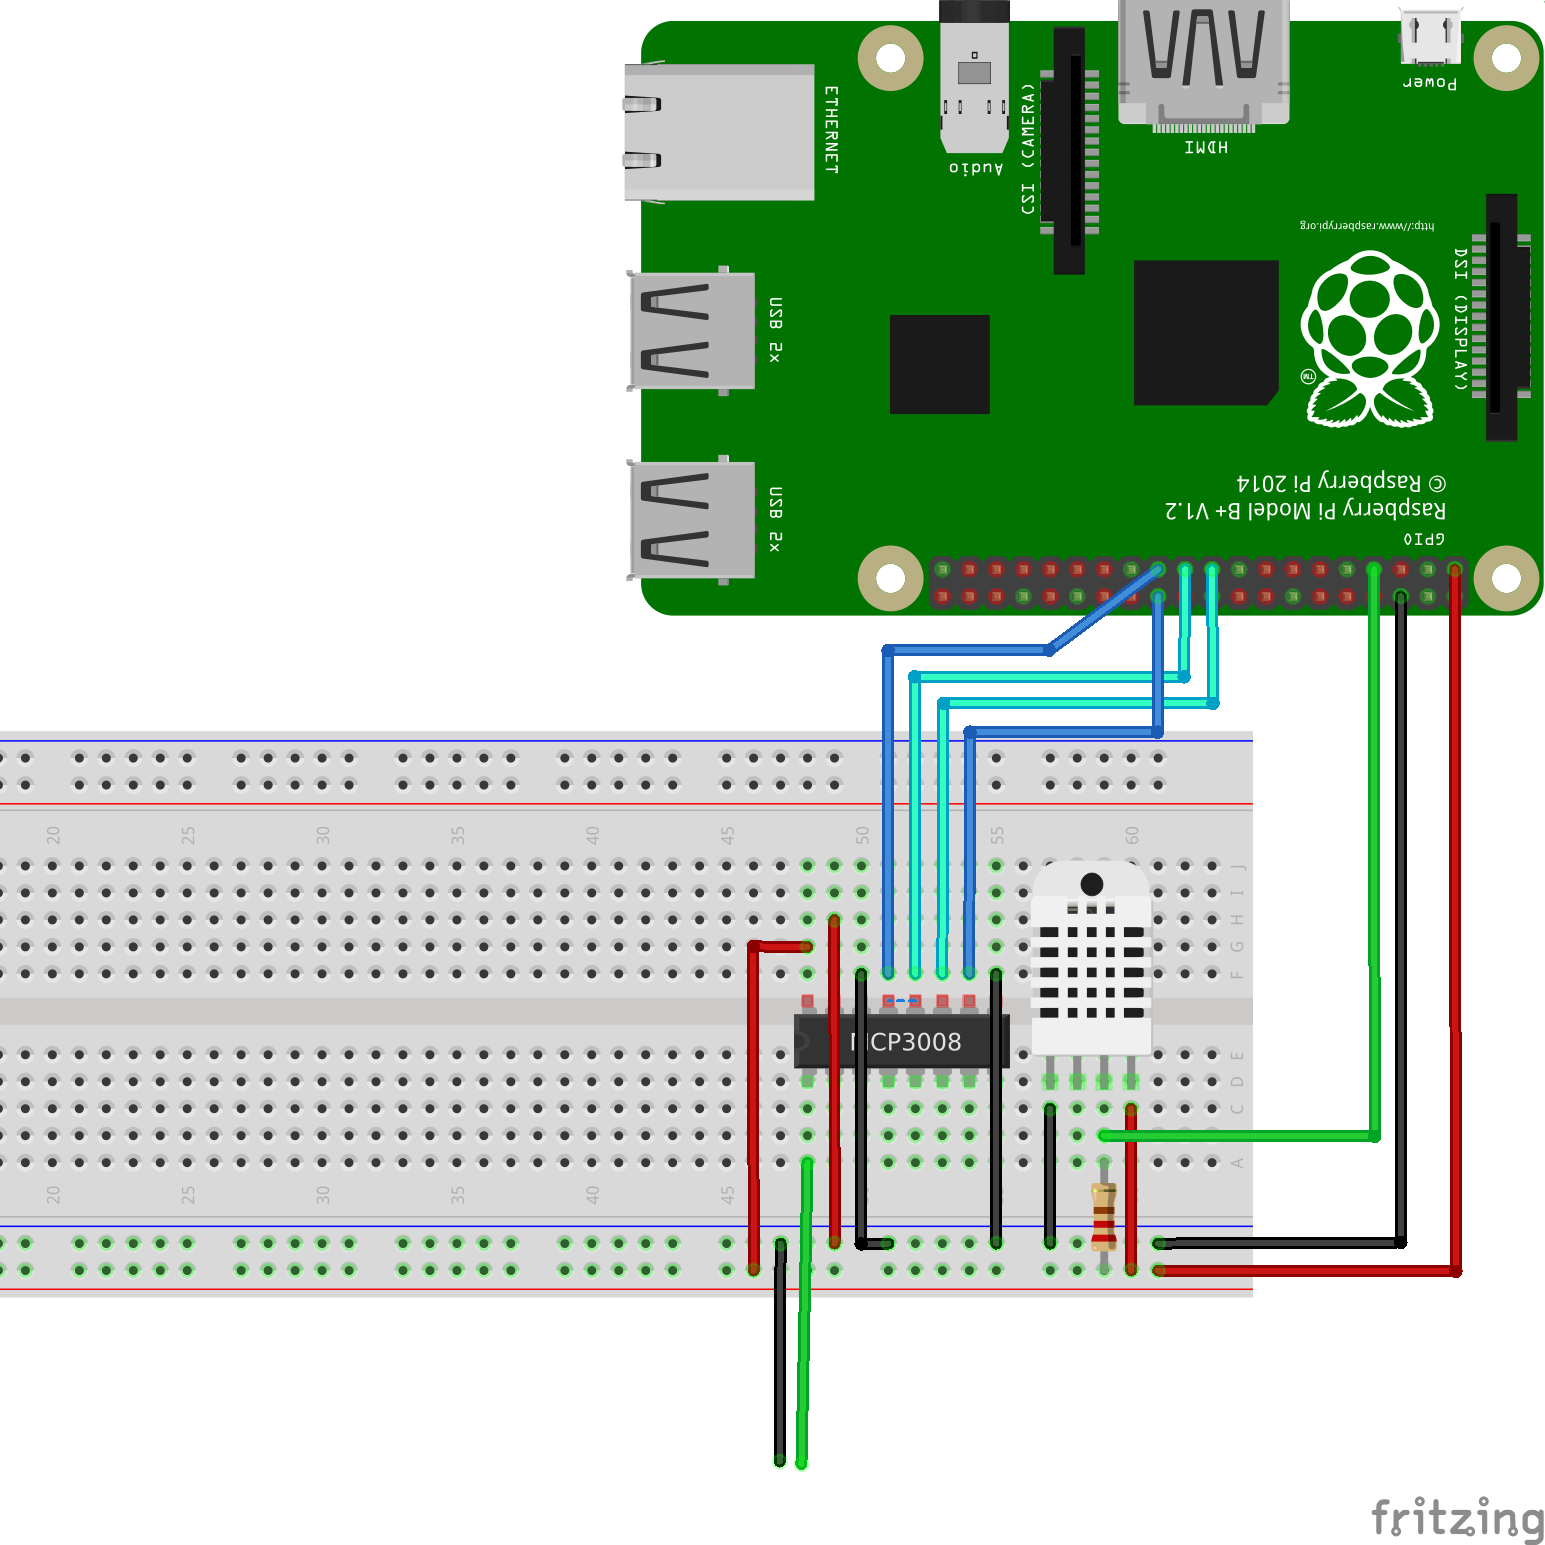
\includegraphics[width=15cm,height=15cm]{figures/solar_project_node_diagram.png}
		\caption{Diagrama del nodo}
	\end{center}
	
	\label{node-diagram}
\end{figure}

%%Falta hablar de los logs que hace el nodo